\section{User Interface Overview}
The main idea behind the RMA user interface (UI) is to provide all the necessary information to the user without the need to open or switch to extra windows. Also, the previous rotable movement user interface (i.e. iRMS) was work order centric. However, the main aspects of the rotable life cycle management are workshops, wagons, rotables and now movement advices -- this is reflected in the UI presented in this document.

The current version of the document describes only the PNL user UI perspective for working with a specific workshop. There is also a Contractor user UI perspective, which is yet to be included. \hyperref[fig:01-complete-ui]{Figure~\ref*{fig:01-complete-ui}} depicts the PNL user UI perspective, which has all available controls open and present in one widow.

\begin{figure}[!h]
\centering
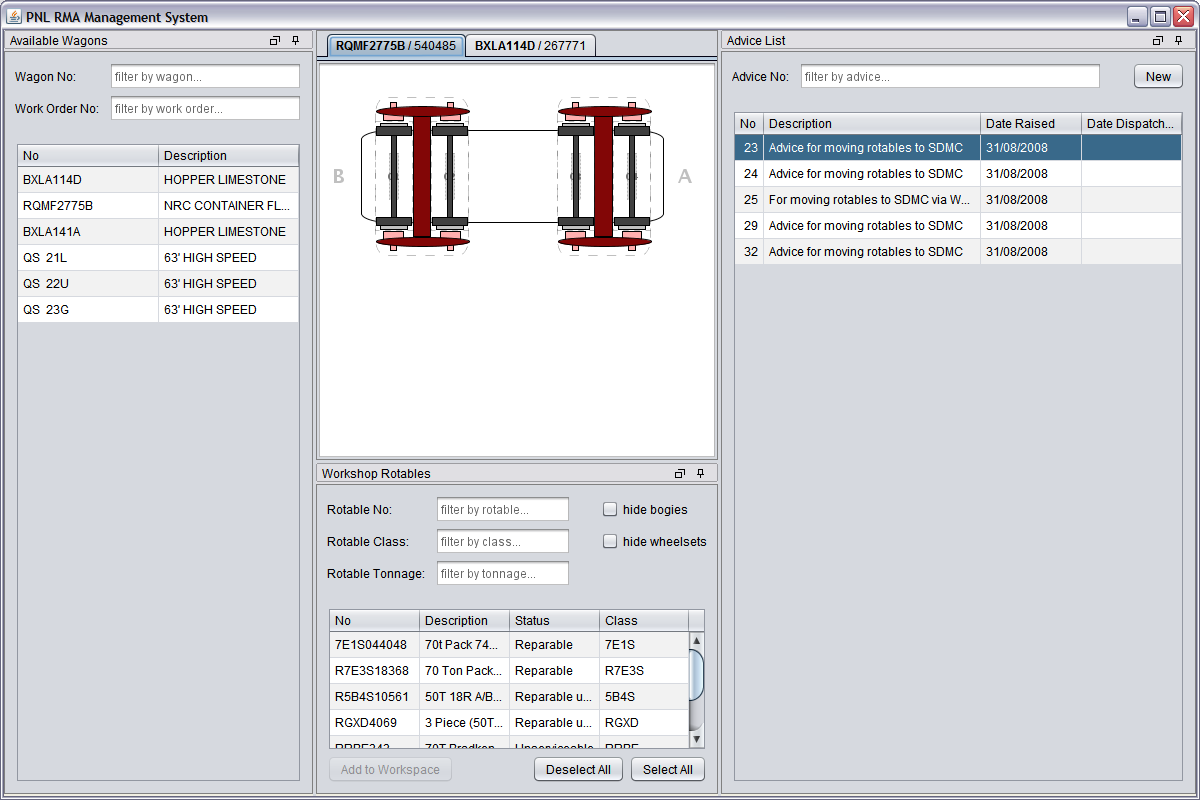
\includegraphics[scale=0.37]{chapters/01-user-interface/images/01-complete-ui.png}
\caption{PNL Perspective}\label{fig:01-complete-ui}
\end{figure}

There are four sections in this window:
\begin{itemize}
	\item Available Wagons -- sub-panel where the user can quickly navigate and review wagon related information; it is used for choosing the wagons to be used in fitment/defitment operations.
	\item Workshop Workspace -- the main area, similar to iRMS, where the user performs interactive fitment/defitment operations and placement of rotables on a movement advice.
	\item Rotable Selection -- sub-panel where the user selects those rotables from the workshop that are to be added into the workspace for movement operations.
	\item Advice Selection and Creation -- sub-panel where user can navigate between available movement advices and perform related operations (rotable placement, dispatch, receiving).
\end{itemize}
The UI has been designed to reduce the number of actions the user needs to undertake to perform operations on rotables. For instance, if there is a movement advice awaiting to be receipted and also there is a wagon that can be fitted with rotables from that advice, user can simply locate the advice and receive required rotables directly into the workspace ready for fitment. So, there is no necessity to first receive rotables from advice into a workshop, then select needed ones for fitment and place them into a workspace. At the same time, if user needs only to receive rotables s/he can easily perform just that operation.

All sub-panels are equipped with intuitive filtering capabilities using autocompleters with multi-valued selection and wild card support. This provides an easy way to reduce the amount of available data and efficiently find the required information. The resultant grids are sortable, which further improves information accessibility.
\\\\
The next sections discuss sub-panels in greater details.
\clearpage

\subsection{Wagon Selection}
When working with the rotable life cycle, the user should know either the list (one and more) of wagons that need to be processed (i.e. fitted/defitted), or a list of work orders against those wagons. The \emph{Available Wagons} sub-panel highlighted in \hyperref[fig:02-available-wagons]{Figure~\ref*{fig:02-available-wagons}} provides an easy way to locate the required wagons.

Only those wagons with active work orders for the specified workshop are displayed. The displayed list of wagons may still be too large to efficiently find the required ones. In order to overcome this, the sub-panel includes two filtering criteria -- by wagons and work orders. The filtering controls are autocompleters and support multiple values. So, the user can either type the required values or look'em up. When the user start's typing, the information in the grid is automatically filtered, so the user does not need to enter the whole wagon or work order number.
\begin{figure}[!h]
\centering
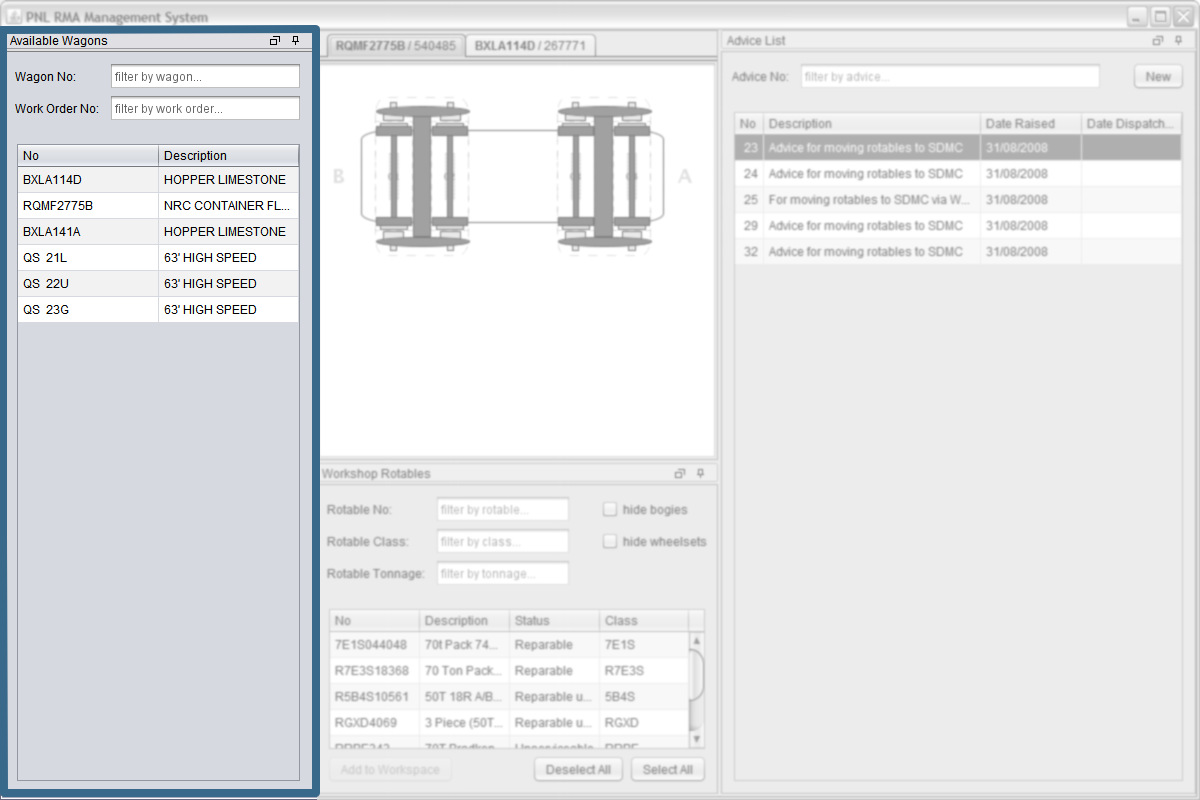
\includegraphics[scale=0.37]{chapters/01-user-interface/images/02-available-wagons.png}
\caption{List of Available Wagons}\label{fig:02-available-wagons}
\end{figure}

Our analysis of the current data suggests that there are situations where the wagons may have several fitment/defitment related active work orders in the same workshop. Therefore, when selecting a wagon to be added to the workspace it is necessary to specify one of the related work orders. The wagon grid provides the \emph{Wagon Details} view as a row expansion, which can be activated by selecting a row with a required wagon. \hyperref[fig:03-available-wagons-expanded]{Figure~\ref*{fig:03-available-wagons-expanded}} depicts the Wagon Details view displaying related work orders. Button \emph{Add to Workspace} should be used for adding wagons to the workspace. It becomes enabled when one of the present work orders is selected. When there is only one work order this button is automatically enabled, saving the user the extra click.

\begin{figure}[!h]
\centering
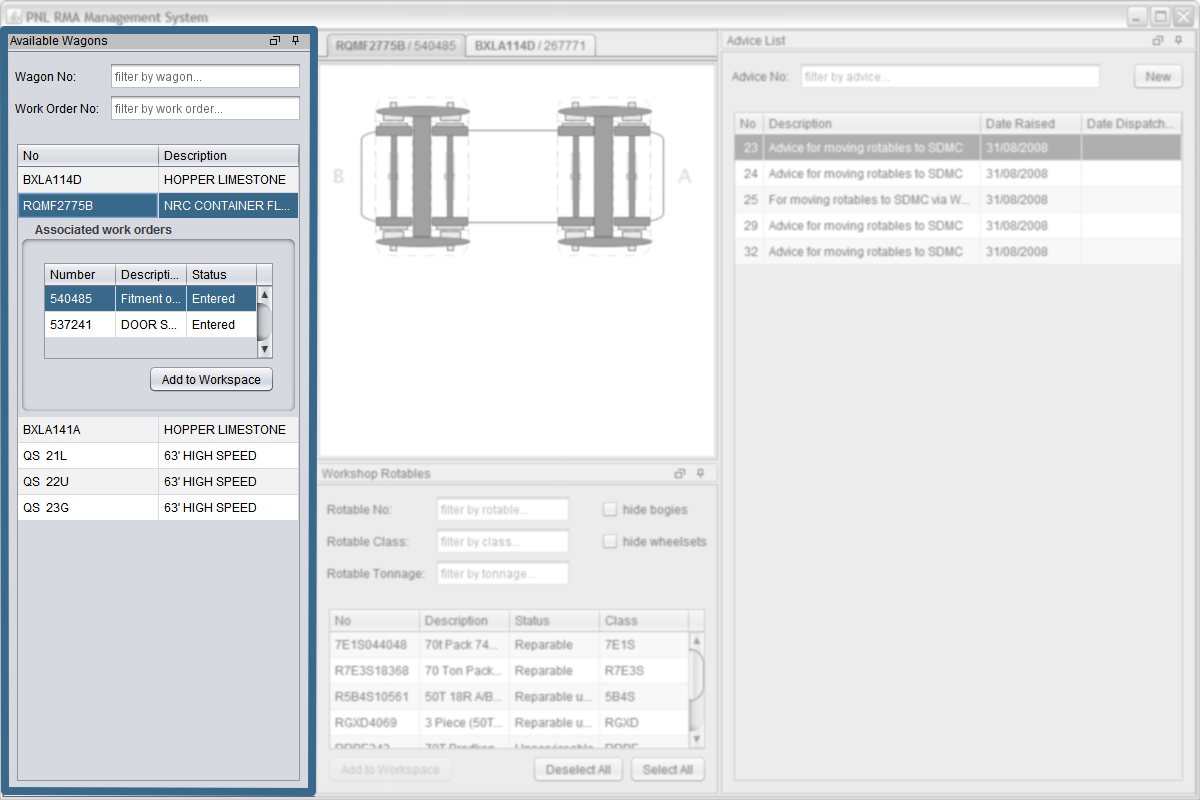
\includegraphics[scale=0.37]{chapters/01-user-interface/images/03-available-wagons-expanded.png}
\caption{Wagon Details}\label{fig:03-available-wagons-expanded}
\end{figure}

\clearpage

\subsection{Workshop Workspace}

\emph{Workshop Workspace} is an area (refer~\hyperref[fig:08-workspace]{Figure~\ref*{fig:08-workspace}}) where the user performs interactive rotable operations such as fitment, defitment and placement onto a movement advice. It is based on the iRMS functionality, but enhances them to the next level, striving to improve the user experience by simplifying the interaction. For example, the workspace features multiple rotable selection in the various operations (e.g. placement onto a movement advice).

Also, the iRMS user is often overloaded with information -- several widgets for different workshops, rotables available in the workshop etc. The workspace has been designed to contain only items requested by the user -- a wagon selected by the user and only those rotables from the workshop and/or movement advices that the user specifically added to the workspace.

The workspace supports tabsheets to enable the user to work on several wagons -- each in a separate tab. The tab caption provides information about the included wagon, as well as the related work order specified when adding wagon to the workspace.

\begin{figure}[!h]
\centering
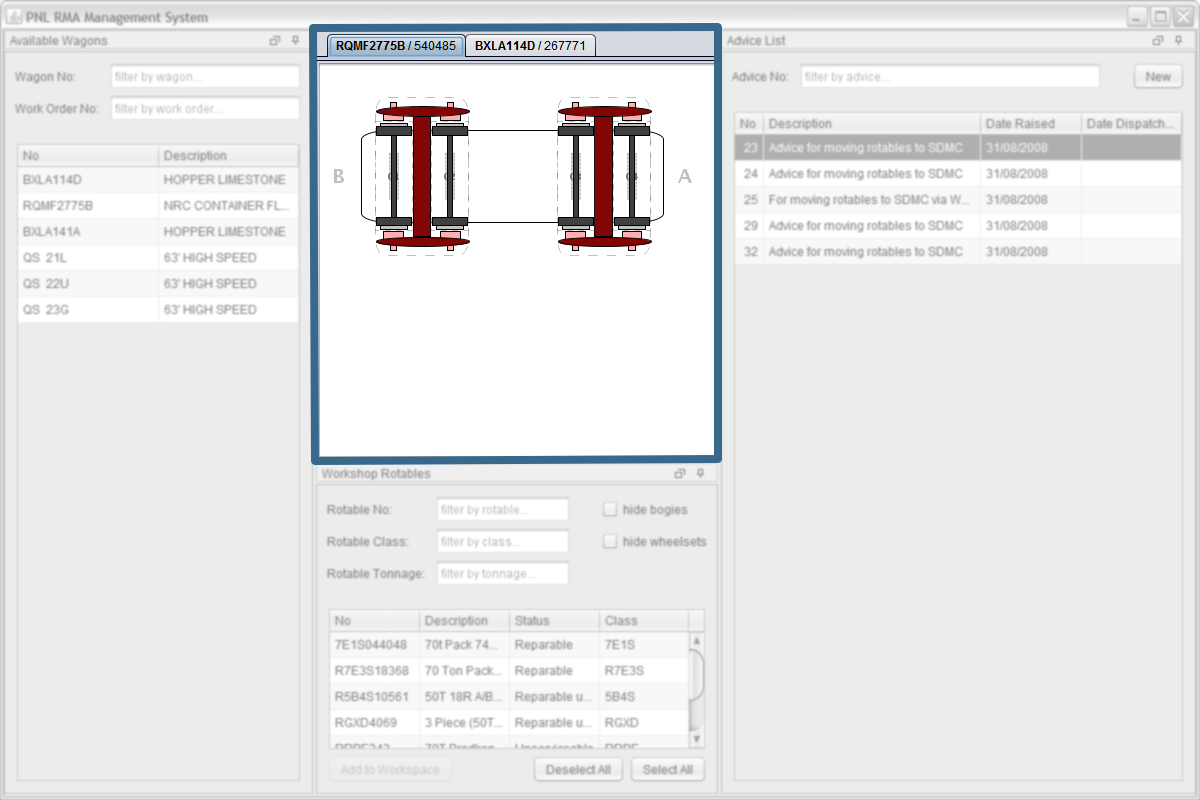
\includegraphics[scale=0.37]{chapters/01-user-interface/images/08-workspace.png}
\caption{Workshop Rotables}\label{fig:08-workspace}
\end{figure}

\clearpage

\subsection{Rotable Selection}

When a wagon is added to the workspace there are no rotables there that could be used for fitment. In order to locate and add necessary rotables to the workspace the \emph{Workshop Rotables} sub-panel (refer~\hyperref[fig:05-rotables-in-workshop-sorted-by-class-with-autocompleter]{Figure~\ref*{fig:05-rotables-in-workshop-sorted-by-class-with-autocompleter}}) should be used. It includes only those rotables that are compatible with the current wagon's hierarchy and reside in the declared workshop.  The user can use filtering criteria to easily locate the required rotables. As for any grid in the application, the displayed rotables can be sorted by any of the columns in both descending and ascending order. The user may select one or more rotables in the grid and add them to the workspace by actioning the \emph{Add to Workspace} button.

\begin{figure}[!h]
\centering
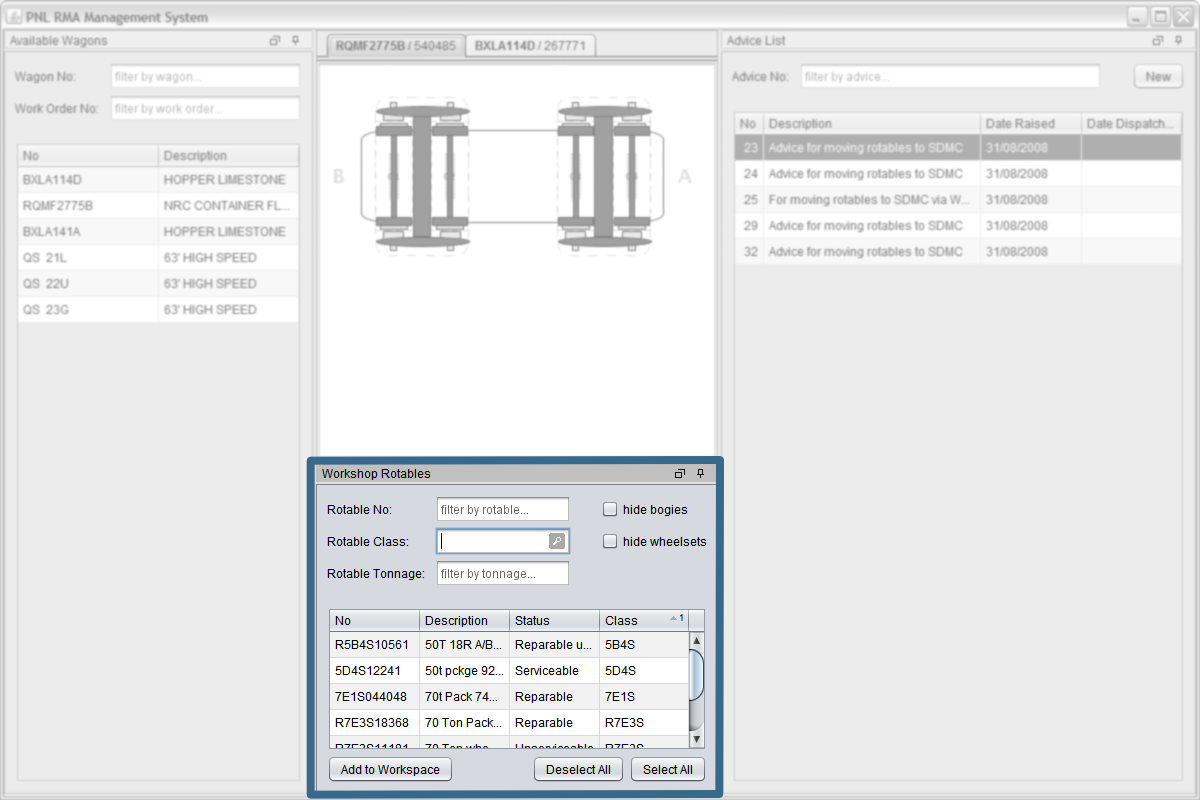
\includegraphics[scale=0.37]{chapters/01-user-interface/images/05-rotables-in-workshop-sorted-by-class-with-autocompleter.png}
\caption{Workshop Rotables}\label{fig:05-rotables-in-workshop-sorted-by-class-with-autocompleter}
\end{figure}

\clearpage

\subsection{Advice Selection and Creation}

The PNL user UI perspective supports movement advice operations such as receiving/placing of rotables from/onto an advice as well as advice dispatch and the creation of a new RMA. All this is provided by the \emph{Advice List} sub-panel (refer~\hyperref[fig:07-advice-list-expanded]{Figure~\ref*{fig:07-advice-list-expanded}}), which displays non-dispatched advices initiated within PNL, and dispatched, but not fully received advices initiated at the Contractor workshop. Similar to the \emph{Available Wagons} sub-panel, it supports row expansion where the movement advice details are displayed. The filtering criterion caters for easy pre-filtering of the required advices.
\\\\
As was mentioned before, the user can receive rotables from a movement advice into the current workshop (only if it matches the receiving workshop) with an option for those rotables to be automatically added to the workspace.

\begin{figure}[!h]
\centering
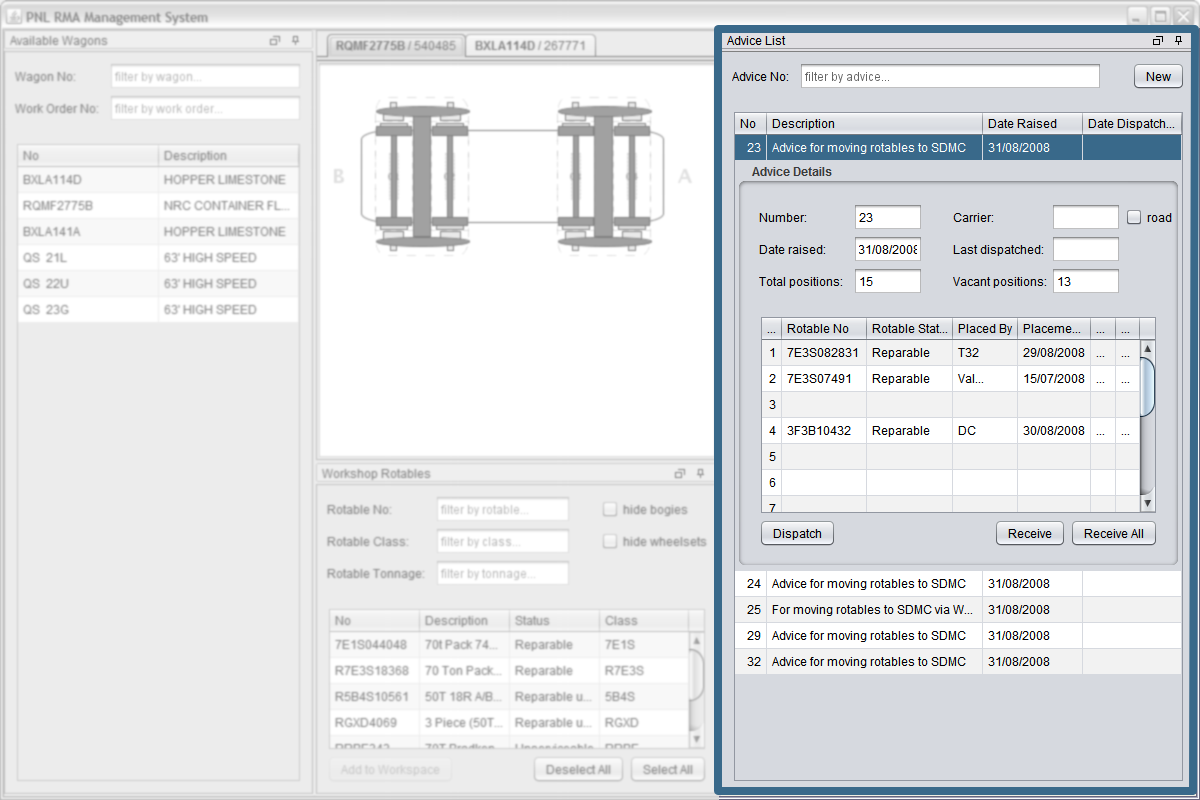
\includegraphics[scale=0.37]{chapters/01-user-interface/images/07-advice-list-expanded.png}
\caption{Advice Details}\label{fig:07-advice-list-expanded}
\end{figure}

\clearpage

\subsection{Layout Configuration with Docking Support}
An astute reader probably is already wondering how convenient it would be to have all those sub-panels in one window at the same time, and to be able to comfortably interact with rotables in such a small workspace... The answer to this is... not 42, but \emph{docking support}. Any sub-panel, except the workspace, can be docked to any side of the window and made invisible when it is not being used. For example, once all the relevant wagons are added to the workspace there is no need to have the Available Wagons sub-panel visible. The same is true about other sub-panels. The provided docking functionality supports any custom user layout and hiding of any/all sub-panels, which in turn, become buttons on the window border, and are easily accessible again by clicking or hovering over the related button with a mouse cursor.
\\\\
\hyperref[fig:09-workspace-custom-layout]{Figure~\ref*{fig:09-workspace-custom-layout}} shows a custom sub-panel layout, whereas \hyperref[fig:10-workspace-all-collapsed]{Figure~\ref*{fig:10-workspace-all-collapsed}} shows the window with all sub-panels being collapsed to the left border. Obviously this significantly increases the workspace area allowing it to occupy almost the whole window.

\begin{figure}[!h]
\centering
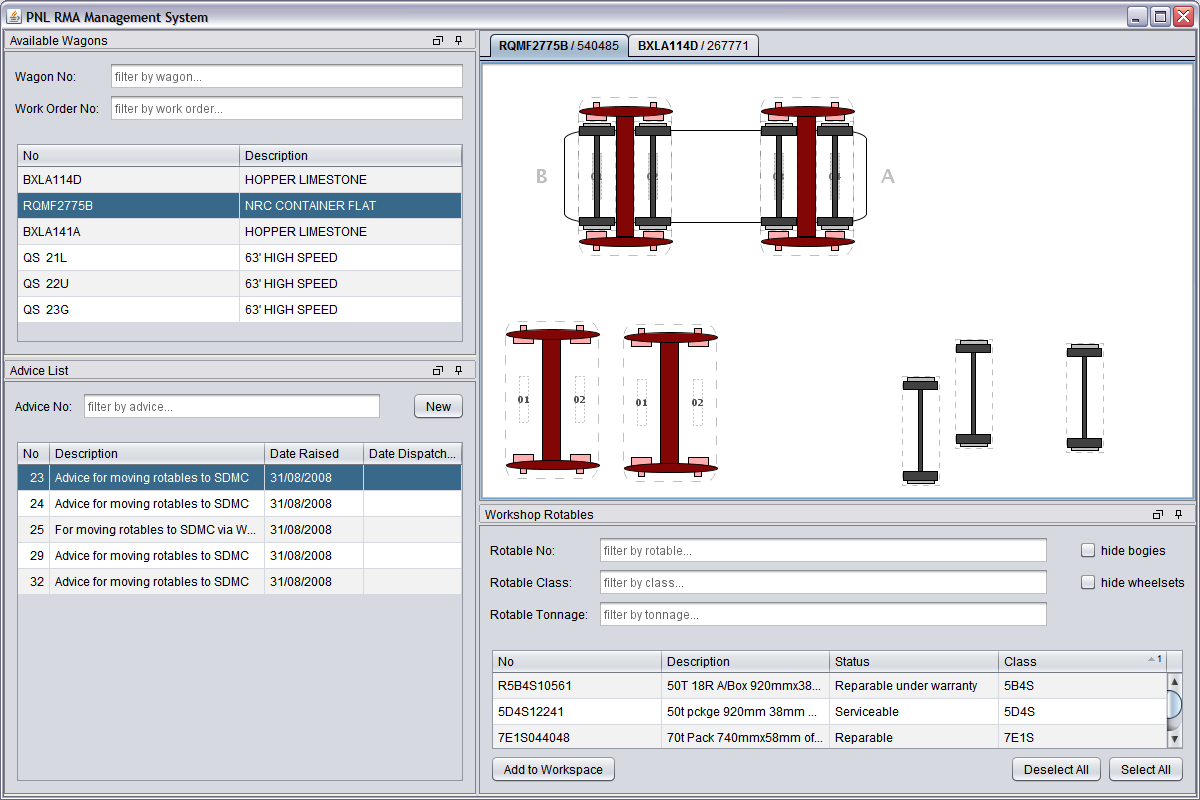
\includegraphics[scale=0.37]{chapters/01-user-interface/images/09-workspace-custom-layout.png}
\caption{Custom Layout}\label{fig:09-workspace-custom-layout}
\end{figure}

\begin{figure}[!h]
\centering
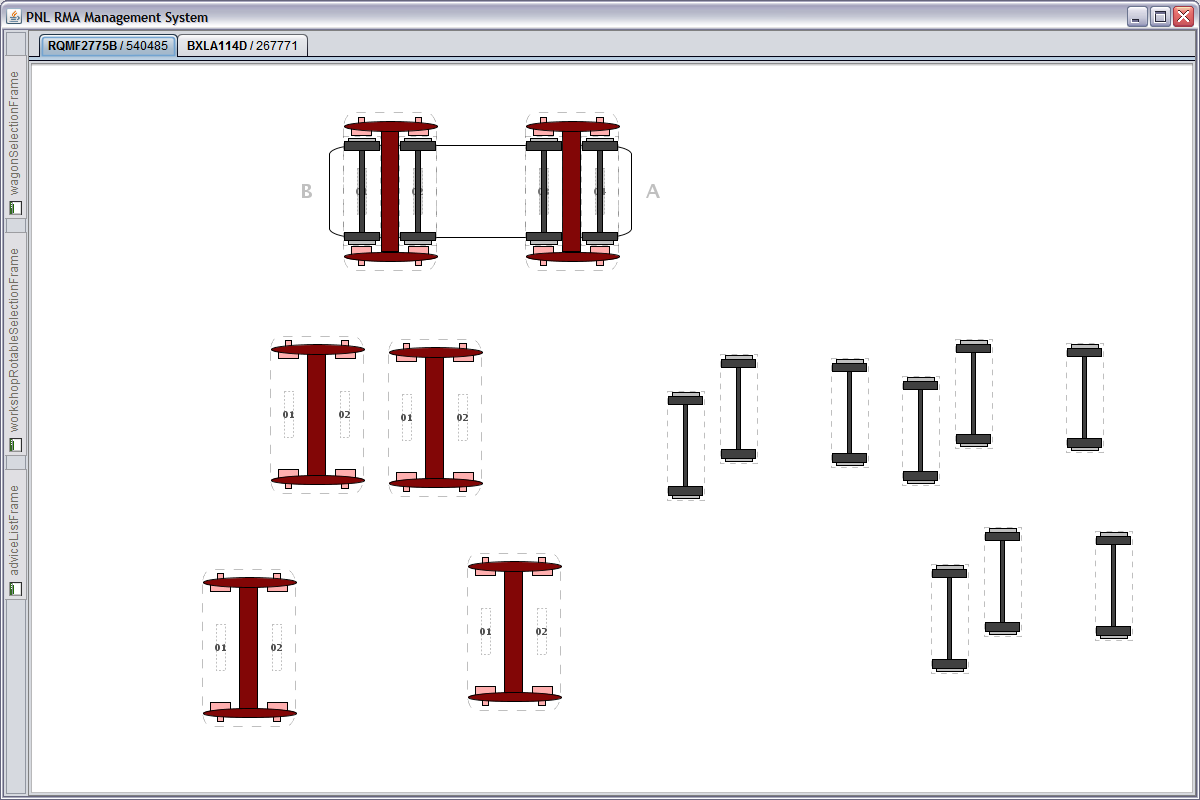
\includegraphics[scale=0.37]{chapters/01-user-interface/images/10-workspace-all-collapsed.png}
\caption{Collapsed Sub-Panels}\label{fig:10-workspace-all-collapsed}
\end{figure}
